\section{Auswertung}
\label{sec:Auswertung}

\subsection{Kontrast}
\label{subsec:Kontrast}
Zu Beginn der Auswertung wurde der maximale Kontrast ermitttelt, der dann für die weitere Auswertung verwendet wurde.
Wie in DURCHFÜHRUNG beschrieben, wurden die Messpunkte aufgenommen und mithilfe von FORMEL wurde der Kontrast bestimmt.
Die Ergebnisse sind in \ref{tab:Kontrast} zu finden.
Der maximale Kontrast mit $0.97$ wurde bei $135°$ bestimmt.
Somit wurde der Polarisatiosfilter auf $135°$ gestellt und mit der Versuchsdurchführung und der Auswertung weitergearbeitet.

\noindent
Desweiteren wird mit den Messwerten eine Ausgleichsrechnung mit python durchgeführt.
Der Kontrast $K$ kann mit folgender Funktion beschrieben werden:
\begin{equation*}
  K = A \cdot | \cos(\Phi)\sin(\Phi) | \, .
\end{equation*}
Durch die Ausgleichsrechnung wird für $A = 1.89 \pm 0.05$ ermittelt.
Die aufgenommenen Messwerte, sowie die Ausgleichsfunktion sind in \ref{fig:Kontrast_Ausgleich} grafisch abgebildet.

\begin{figure}
  \centering
  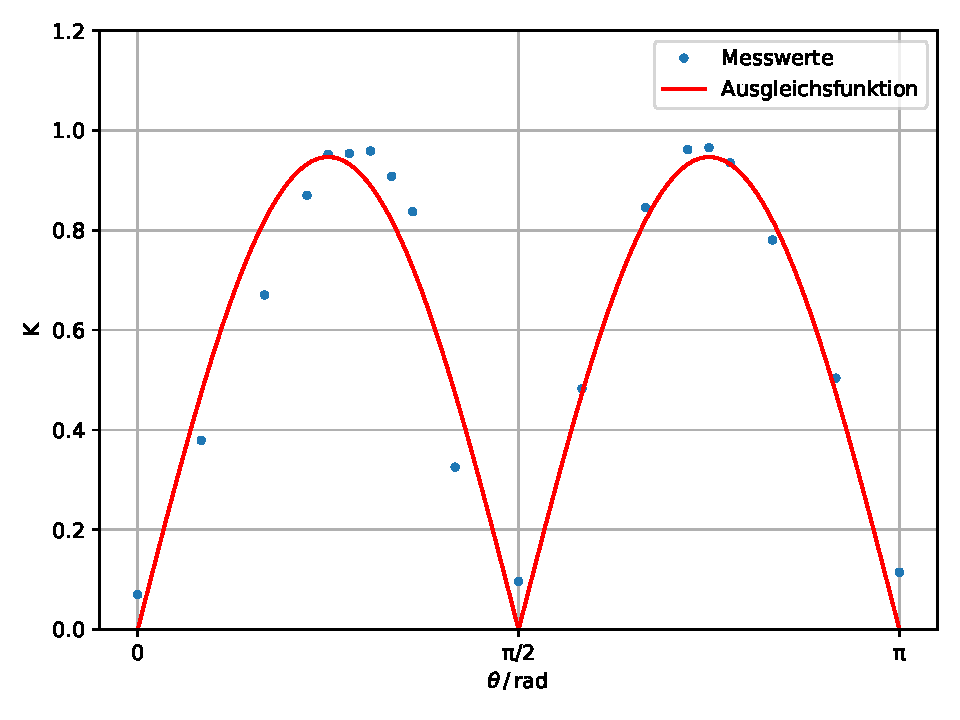
\includegraphics[width=0.6\textwidth]{build/kontrast_ausgleich.pdf}
  \caption{Die aufgenommenen Messwerte zur Ermittlung des Kontrasts und die Ausgleichsrechnung.}
  \label{fig:Kontrast_Ausgleich}
\end{figure}

\begin{table}
  \centering
  \caption{Aufgenommene Messwerte zur Kontrastmessung, sowie der jeweilige Kontrastwert.}
  \label{tab:Kontrast}
  \begin{tabular}{c c c c}
    \toprule
    $\Phi / ° $ & $U_{\text{min}} / \si{\volt}$ & $U_{\text{max}} / \si{\volt}$ & $K$ \\
    \midrule
    0     &  0.86  &  0.99  & 0.07  \\
    15    &  0.36  &  0.80  & 0.38  \\
    30    &  0.14  &  0.71  & 0.67  \\
    40    &  0.05  &  0.72  & 0.87  \\
    45    &  0.02  &  0.82  & 0.95  \\
    50    &  0.02  &  0.85  & 0.95  \\
    55    &  0.02  &  0.96  & 0.96  \\
    60    &  0.05  &  1.04  & 0.91  \\
    65    &  0.10  &  1.13  & 0.84  \\
    75    &  0.58  &  1.14  & 0.33  \\
    90    &  0.84  &  1.02  & 0.10  \\
    105   &  0.60  &  1.72  & 0.48  \\
    120   &  0.22  &  2.63  & 0.85  \\
    130   &  0.06  &  3.08  & 0.96  \\
    135   &  0.05  &  2.85  & 0.97  \\
    140   &  0.10  &  3.00  & 0.94  \\
    150   &  0.32  &  2.60  & 0.78  \\
    165   &  0.62  &  1.88  & 0.50  \\
    180   &  0.77  &  0.97  & 0.11  \\
    \bottomrule
  \end{tabular}
\end{table}

\subsection{Brechungsindex von Glas}
\label{subsec:n_Glas}
Um den Brechungsindex von Glas zu bestimmen, wurden die Intensitätsmaxima $M$, wie in der DURCHFÜHRUNG beschrieben, aufgenommen.
Mithilfe der FORMEL wurde der Brechungsindex bestimmt.
Dabei beträgt die Dicke der Platten $T = \SI{1}{\milli\metre}$, die Wellenlänge des Lasers $\lambda = \SI{632.990}{\nano\metre}$ und $\delta = 10°$, da die beiden Platten jeweils um $\delta$ geneigt waren \cite{anleitung}.
Die aufgenommenen Messwerte sowie der jeweils ermittelte Brechungsindex sind in \ref{tab:Glas} zu finden.
Im Mittel beträgt der ermittelte Brechungsindex für Glas $n_\text{Glas} = 1.0001079364890089$.


\begin{table}
  \centering
  \caption{Aufgenommene Messwerte zur Bestimmung des Brechungsindex von Glas, sowie der ermittelte Brechungsindex.}
  \label{tab:Glas}
  \begin{tabular}{c c c}
    \toprule
    Durchgang & M & $n_\text{Glas}$ \\
    \midrule
    1    &   30    &   1.00009496\\   
    2    &   35    &   1.00011079\\   
    3    &   36    &   1.00011395\\   
    4    &   36    &   1.00011395\\   
    5    &   35    &   1.00011079\\   
    6    &   35    &   1.00011079\\   
    7    &   35    &   1.00011079\\   
    8    &   36    &   1.00011395\\   
    9    &   31    &   1.00009812\\   
    10   &   32    &   1.00010129\\   
    \bottomrule
  \end{tabular}
\end{table}

\subsection{Brechungsindex von Luft}
\label{subsec:n_Luft}
Zur Bestimmung des Brechungsindex von Luft wurden die Messwerte, wie in DURCHFÜHRUNG beschrieben, aufgenommen und mithilfe von FORMEL ermittelt.
Die Länge der Gaskammer beträgt $L = \SI[separate-uncertainty = true]{100(1)}{\milli\metre}$ \cite{anleitung} und die aufgenommene Temperatur $T = \SI{21.1}{\celsius}$.
Die aufgenommenen Messwerte sind in \ref{tab:Luft} zu finden.
Der durchschnittliche Brechungsindex für jeden Durchgang ist in \ref{tab:n_luft_mean} aufgelistet.
Für den durchschnittlichen Brechungsindex ohne Haube wurde $n_\text{Luft,ohne} = 1.0001703 \pm 0.0000017 $ und mit Haube $n_\text{Luft,ohne} =  1.0001622 \pm 0.0000016 $.

\begin{table}
  \centering
  \caption{Aufgenommene Messwerte zur Bestimmung des Brechungsindex von Luft.}
  \label{tab:Luft}
  \begin{tabular}{c c c c c}
    \toprule
    & \multicolumn{2}{c}{Durchgänge ohne Haube} & \multicolumn{2}{c}{Durchgänge mit Haube} \\
    \cmidrule(lr){2-3} \cmidrule(lr){4-5}
    $p / \si{\milli\bar}$ \\
    \midrule
    50    &   4    &   5    &   2     &    2   \\
    100   &   6    &   7    &   4     &    4   \\
    150   &   8    &   10   &   7     &    10  \\
    200   &   10   &   122  &   9     &    12  \\
    250   &   12   &   14   &   11    &    14  \\
    300   &   14   &   16   &   13    &    21  \\
    350   &   17   &   18   &   15    &    23  \\
    400   &   20   &   20   &   17    &    25  \\
    450   &   23   &   22   &   19    &    27  \\
    500   &   25   &   24   &   21    &    29  \\
    550   &   28   &   26   &   24    &    31  \\
    600   &   32   &   29   &   26    &    34  \\
    650   &   36   &   31   &   28    &    36  \\
    700   &   39   &   33   &   30    &    38  \\
    750   &   42   &   35   &   32    &    40  \\
    800   &   44   &   37   &   34    &    42  \\
    850   &   47   &   39   &   36    &    44  \\
    900   &   50   &   41   &   38    &    46  \\
    950   &   54   &   43   &   41    &    48  \\
    100   &   58   &   45   &   42    &    50  \\ 
    \bottomrule
  \end{tabular}
\end{table}

\begin{table}
  \centering
  \caption{Der durchschnittliche Brechungsindex von Luft für jeden Durchgang. Durchgang 1 und 2 wurden ohne Haube durchgeführt, Durchgang 3 und 4 mit.}
  \label{tab:n_luft_mean}
  \begin{tabular}{c c c c}
    \toprule
    Durchgang & M & $n_\text{Glas}$ \\
    \midrule
    1    &  $1.0001801 \pm 0.0000018$ \\   
    2    &  $1.0001605 \pm 0.0000016$ \\   
    3    &  $1.0001823 \pm 0.0000018$ \\   
    4    &  $1.0001421 \pm 0.0000014$ \\   
    \bottomrule
  \end{tabular}
\end{table}